


\section{Simulation Experiments}

\subsection{Experiment Setup}

\textbf{Simulation benchmark.} Though the simulation environments are increasingly realistic nowadays~\citep{makoviychuk2021isaac,xiang2020sapien,todorov2012mujoco,zhu2020robosuite}, a notable gap between simulation and real-world scenarios persists~\citep{Ze2022rl3d,lei2023uni_o4,chen2023visual_dex}. This discrepancy underscores two key aspects: \textit{(a)} the importance of real robot experiments and \textit{(b)} the necessity of large-scale diverse simulation tasks for more scientific benchmarking. Therefore, for simulation experiments, we collect in total \textbf{72} tasks from \textbf{7} domains, covering diverse robotic skills. These tasks range from challenging scenarios like bi-manual manipulation~\citep{chen2022bidexhands}, deformable object manipulation~\citep{li2023dexdeform}, and articulated object manipulation~\citep{bao2023dexart}, to simpler tasks like parallel gripper manipulation~\citep{yu2020metaworld}. These tasks are built with different simulators including MuJoCo~\citep{todorov2012mujoco}, Sapien~\citep{xiang2020sapien}, IsaacGym~\citep{makoviychuk2021isaac}, and PlasticineLab~\citep{huang2021plasticinelab}, ensuring our benchmarking is not limited by the choice of simulator. Tasks in MetaWorld~\citep{yu2020metaworld} are categorized into various difficulty levels
% \textit{easy}, \textit{medium}, \textit{hard}, and \textit{very hard} 
based on \cite{seo2023mwm}. A brief overview is shown in Table~\ref{table:task summary}. \revise{The 3D observations are visualized in Figure~\ref{fig:sim 3d}.}



\begin{figure}[htbp]
    \centering
    \vspace{-0.1in}
    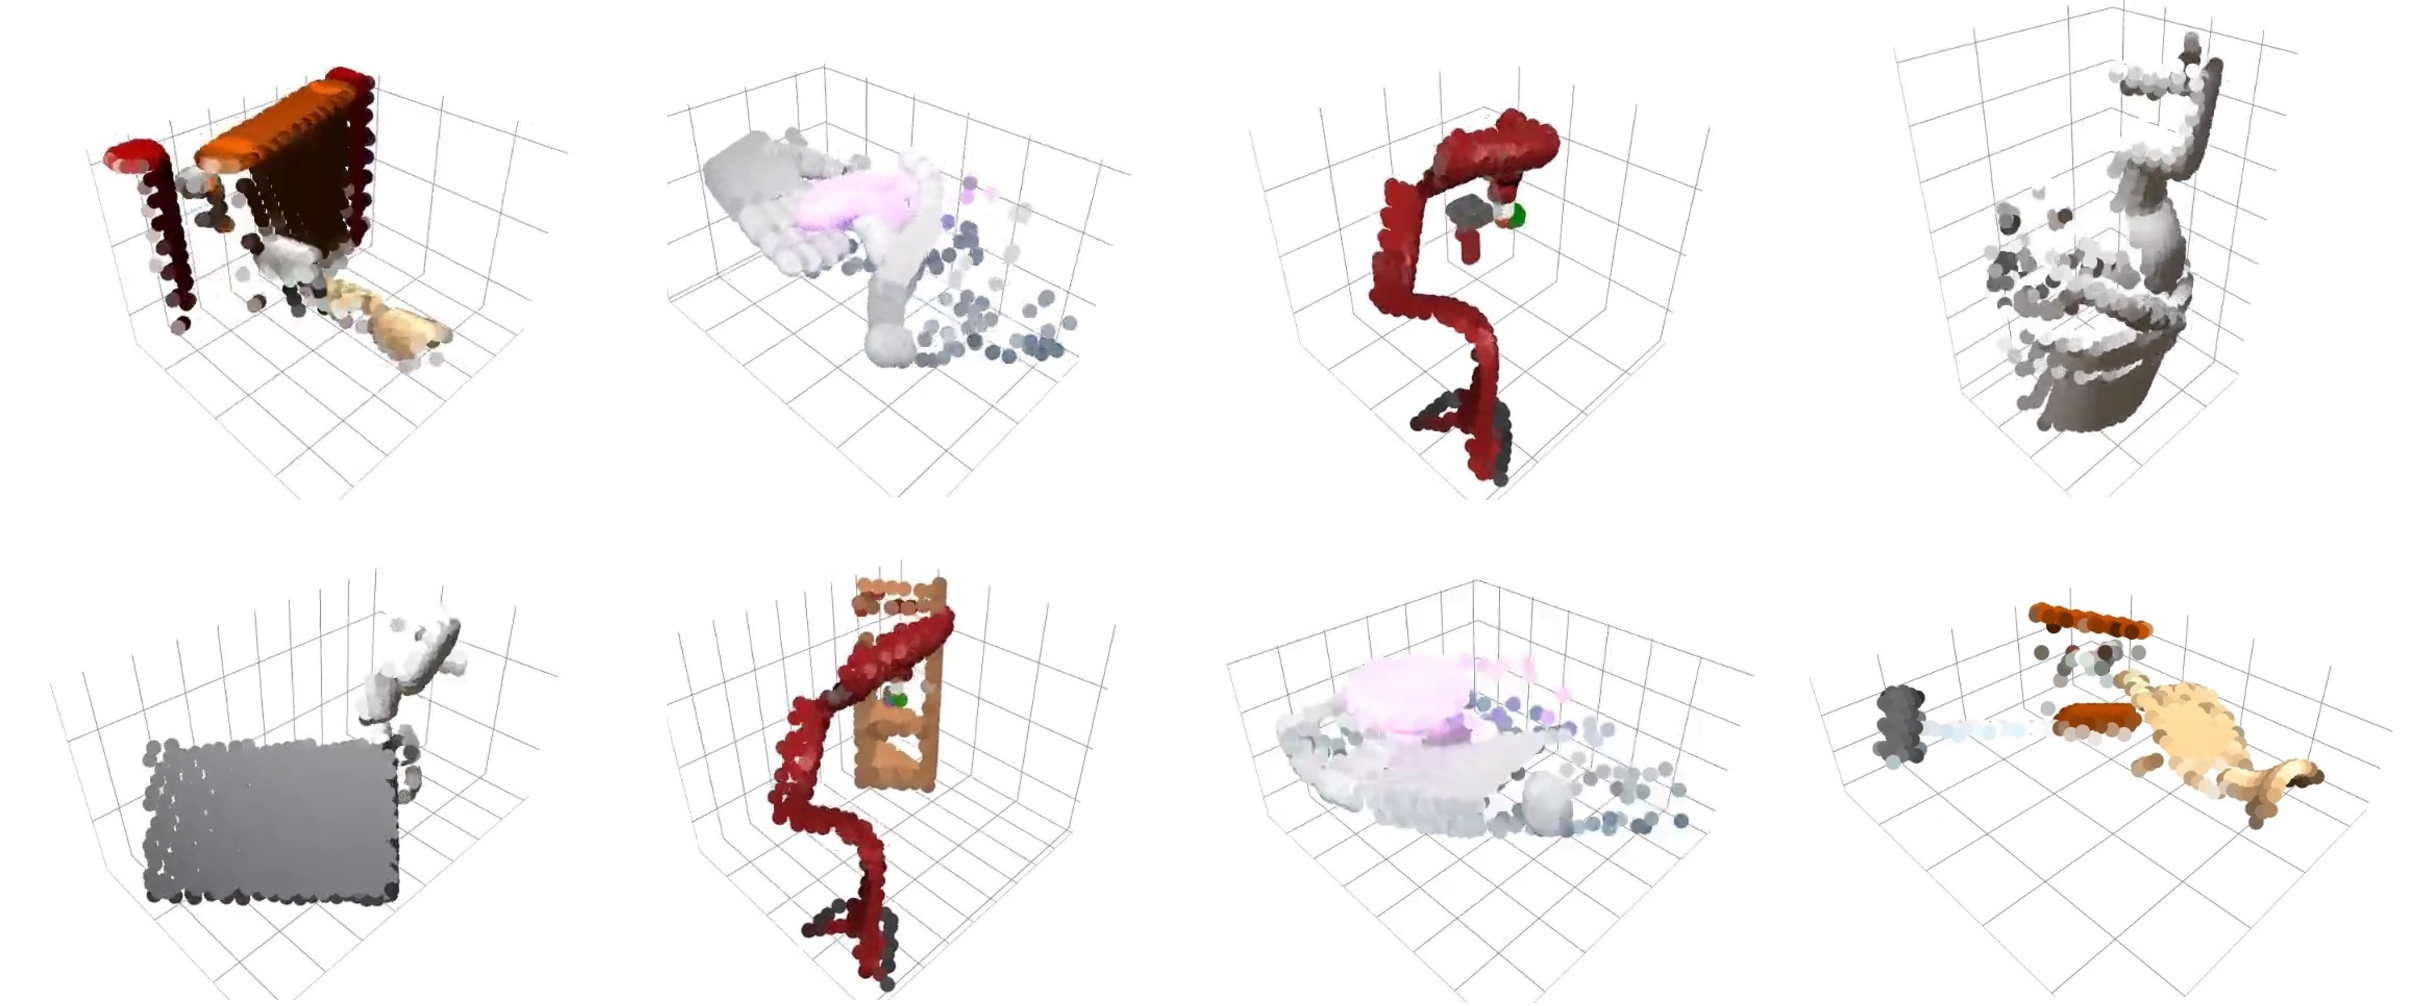
\includegraphics[width=0.5\textwidth]{figures/sim3d.pdf}
    \caption{\textbf{3D visual observations in simulation.} We sample some simulated tasks and show the downsampled point clouds in these tasks.}
    \label{fig:sim 3d}
    \vspace{-0.15in}
\end{figure}

% \textbf{Expert demonstrations} are collected with agents trained by reinforcement learning (RL) algorithms for all the domains except DexDeform, where we use human-teleoperated data. VRL3~\citep{wang2022vrl3} is used for Adroit; BAC~\citep{ji2023bee} is used for MetaWorld; PPO~\citep{schulman2017ppo} is used in all other domains. We generate successful trajectories with RL agents and ensure all imitation learning algorithms are using the same demonstrations. The success rates for experts are given in Appendix~\ref{appendix: full simulation results}.

\textbf{Expert demonstrations.} Human-teleoperated data is used in DexDeform; \revise{Script policies are used in MetaWorld;} Trajectories for other domains are collected with agents trained by reinforcement learning (RL) algorithms, where we use VRL3~\citep{wang2022vrl3} is used for Adroit; PPO~\citep{schulman2017ppo} is used in all other domains. We generate successful trajectories with RL agents and ensure all imitation learning algorithms are using the same demonstrations. The success rates for experts are given in Appendix~\ref{appendix: full simulation results}.


\textbf{Baselines.} The primary focus of this work is to underscore the significance of the 3D modality in diffusion policies. To this end, our main baseline is the image-based diffusion policy~\citep{chi2023diffusion_policy}, simply referred to as \textit{Diffusion Policy}. Additionally, we incorporate comparisons with IBC~\citep{florence2022ibc},  BCRNN~\citep{mandlekar2021robomimic}, and their 3D variations. However, given that these algorithms showed limited effectiveness in our challenging tasks, we evaluate them on only 10 tasks (see Table~\ref{table: compare with more baselines}). We emphasize that the image and depth resolution for all 2D and 3D methods are \textbf{the same} across all experiments, ensuring a fair comparison.








\textbf{Evaluation metric.} We run 3 seeds for each experiment with seed number $0,1,2$. For each seed, we evaluate 20 episodes every 200 training epochs and then compute the average of the highest 5 success rates. We report the mean and std of success rates across 3 seeds.






\begin{table}[t]
\caption{\textbf{Task suite of \ours,} including Adroit~\citep{rajeswaran2017dapg}, Bi-DexHands~\citep{chen2022bidexhands}, DexArt~\citep{bao2023dexart}, DexDeform~\citep{li2023dexdeform}, DexMV~\citep{qin2022dexmv}, HORA~\citep{qi2023hora}, MetaWorld~\citep{yu2020metaworld}, and our real robot tasks.
ActD: the highest action dimension for the domain. \#Demo: Number of expert demonstrations used for each task in the domain. Art: articulated objects. Deform: deformable objects.}
\label{table:task summary}
\vspace{-0.05in}
\resizebox{0.5\textwidth}{!}{%
\begin{tabular}{lcccccccc}
\toprule
\toprule
\multicolumn{7}{c}{\textbf{Simulation Benchmark (72 Tasks)}} \\
\midrule
 Domain & Robo  & Object  & Simulator & ActD & \#Task & \#Demo\\
 
\midrule
\textbf{Adroit} & Shadow & Rigid/Art & MuJoCo & 28 & 3 & 10\\


\textbf{Bi-DexHands} & Shadow & Rigid/Art &  IsaacGym & 52 & 6 & 10\\


\textbf{DexArt} & Allegro & Art & Sapien & 22 & 4 & 100 \\


\textbf{DexDeform} & Shadow & Deform & PlasticineLab & 52 & 6 & 10\\


\textbf{DexMV} & Shadow  & Rigid/Fluid & Sapien & 30 & 2 & 10\\


\textbf{HORA} & Allegro  & Rigid & IsaacGym & 16 & 1 & 100\\



\textbf{MetaWorld} & Gripper & Rigid/Art & MuJoCo & 4 & 50 & 10 \\


\toprule

% \textbf{Summary} & / & / & /  & 78 & / \\


\end{tabular}
}
\resizebox{0.5\textwidth}{!}{%
\begin{tabular}{lcccclcccc}
\multicolumn{6}{c}{\textbf{Real Robot Benchmark (4 Tasks) }} \\
\midrule

Task & Robo & Object &  ActD & \#Demo & Description\\

\midrule
\textbf{Roll-Up} & Allegro & Deform & 22 & 40 & Wrap plasticine to make a roll-up\\

\textbf{Dumpling} & Allegro & Deform & 22 & 40 & Wrap plasticine and pinch with fingers\\

\textbf{Drill} & Allegro & Rigid & 22 & 40 & Grasp the drill and touch the cube\\

% \textbf{Scissors} & Allegro & Art & 22 & 40 & Pick the scissors towards flowers\\

\textbf{Pour} & Gripper & Rigid & 7 & 40 & Pick the bowl, pour, and place \\
\bottomrule
\bottomrule
\end{tabular}
}
% 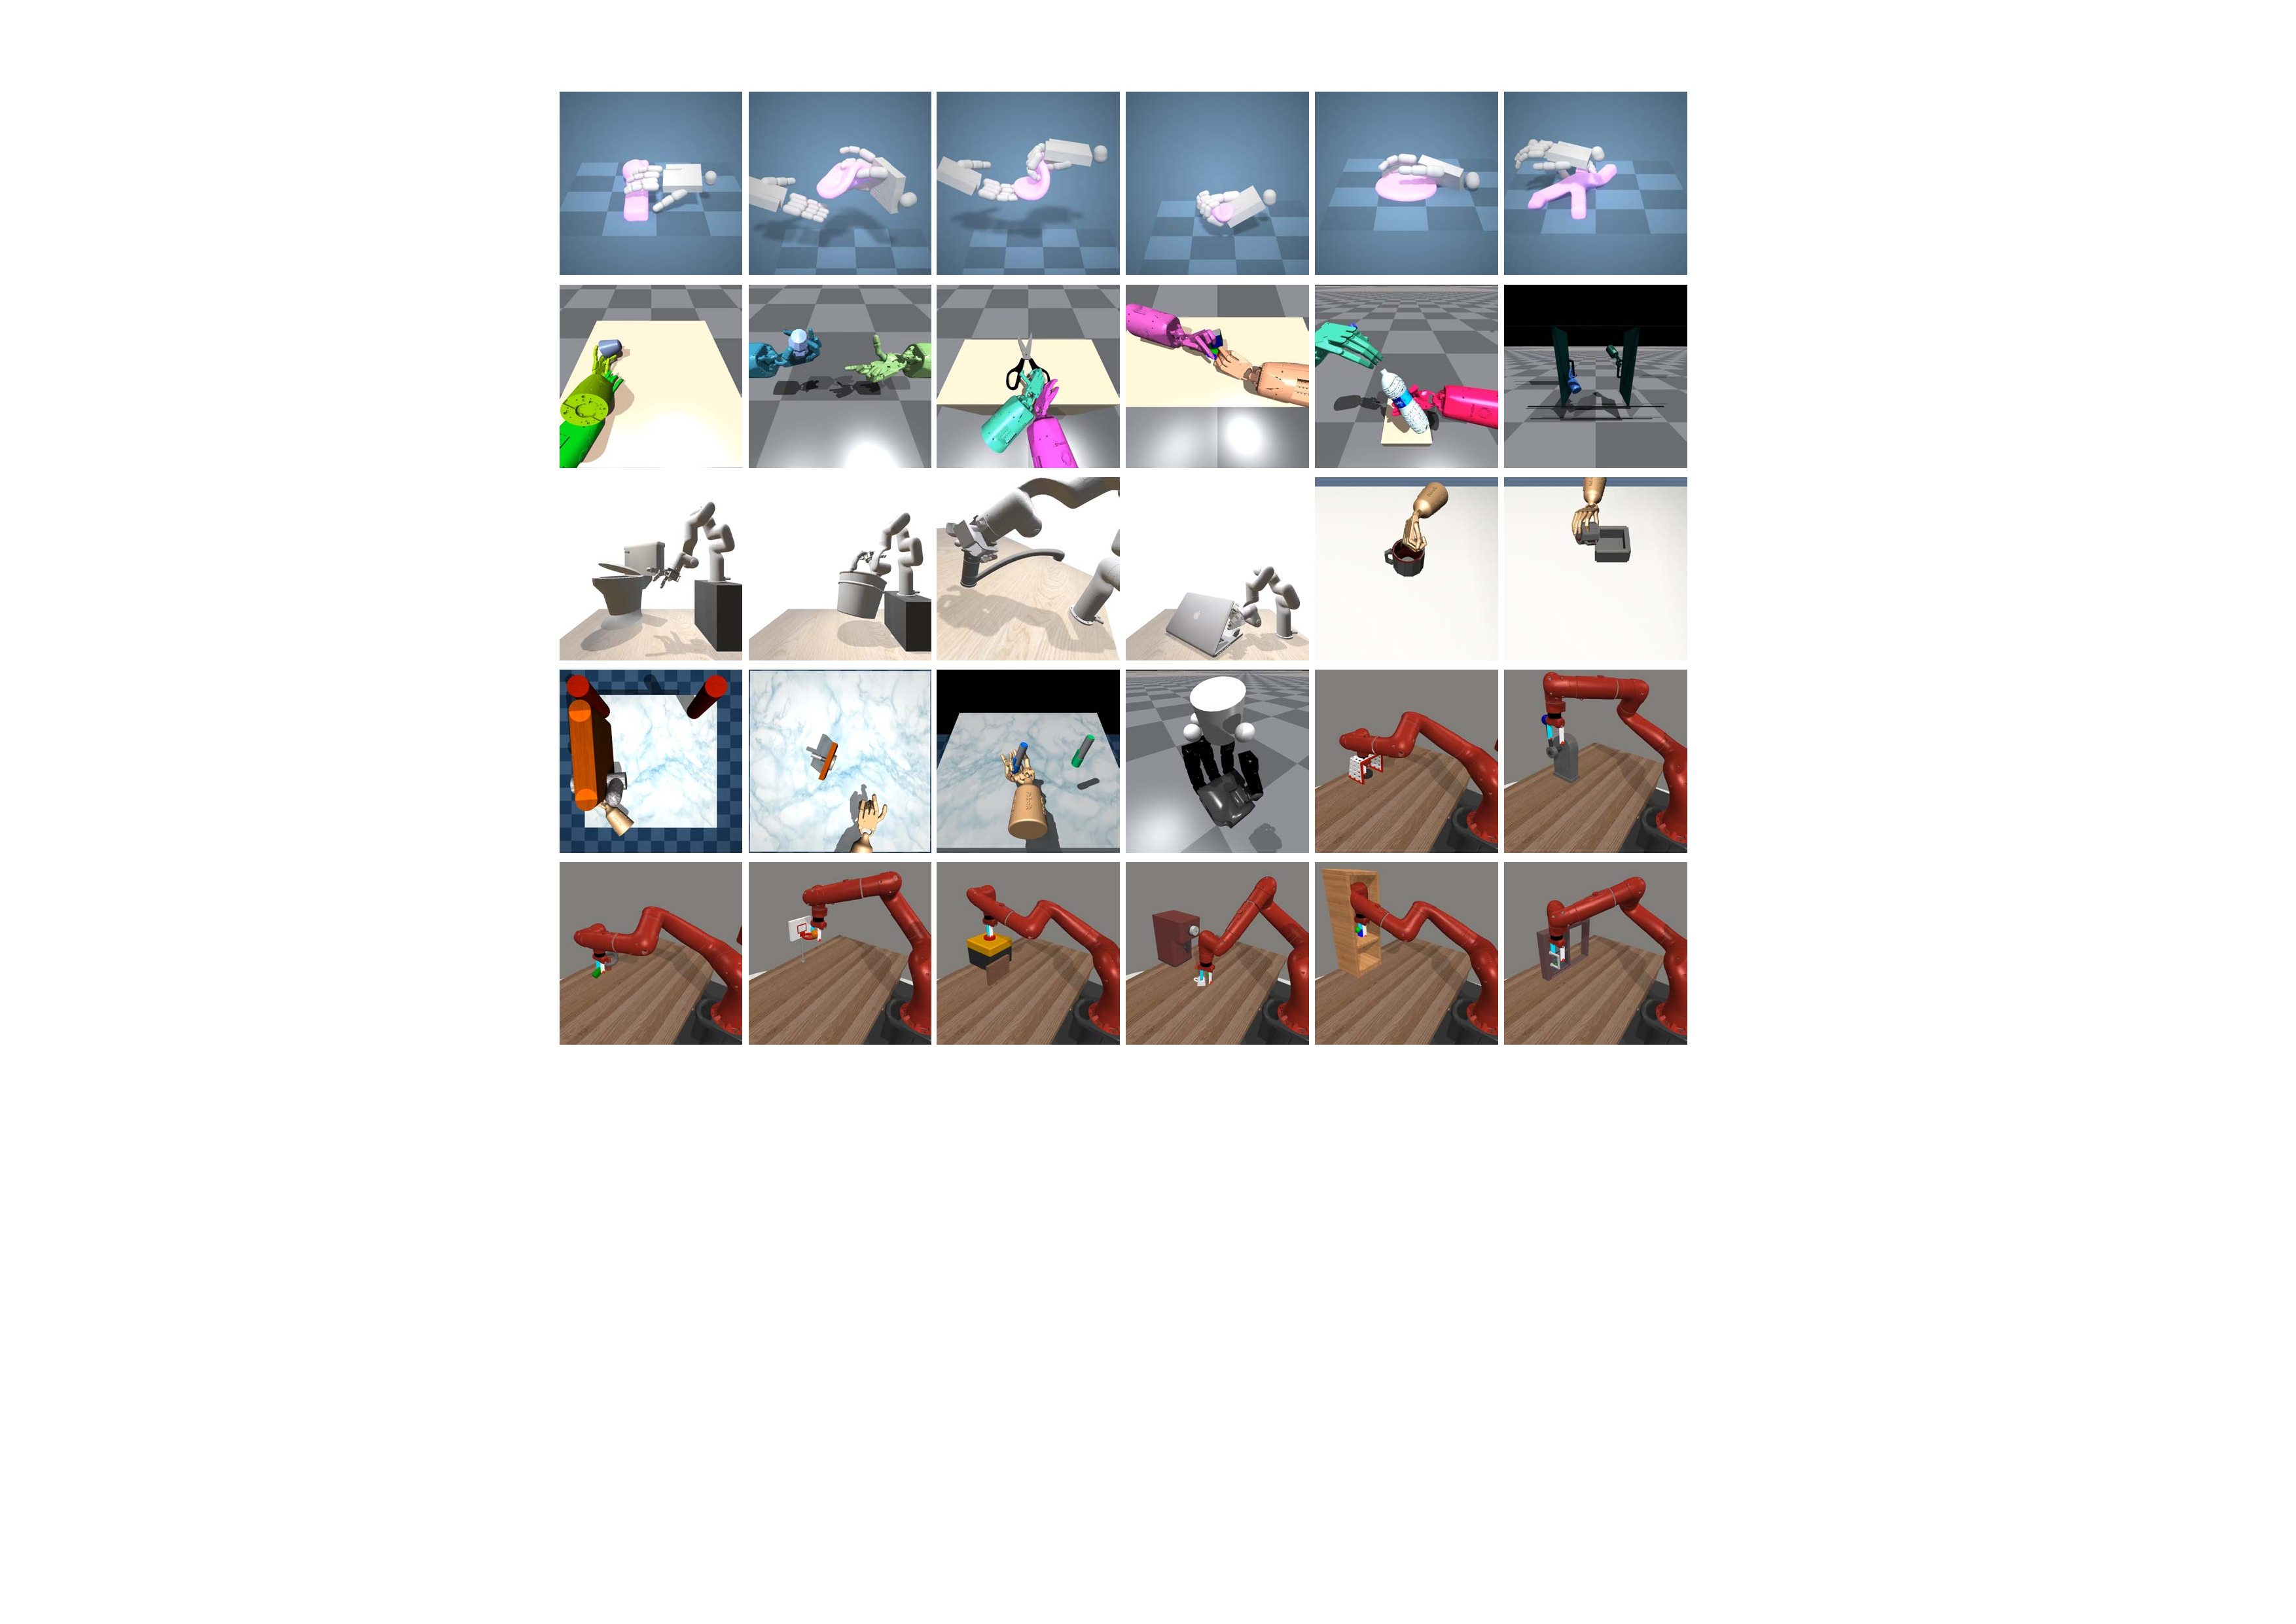
\includegraphics[width=0.5\textwidth]{figures/task_visualization_compress.pdf}
\vspace{-0.2in}
 \end{table}









\begin{figure*}[t]
    \centering
    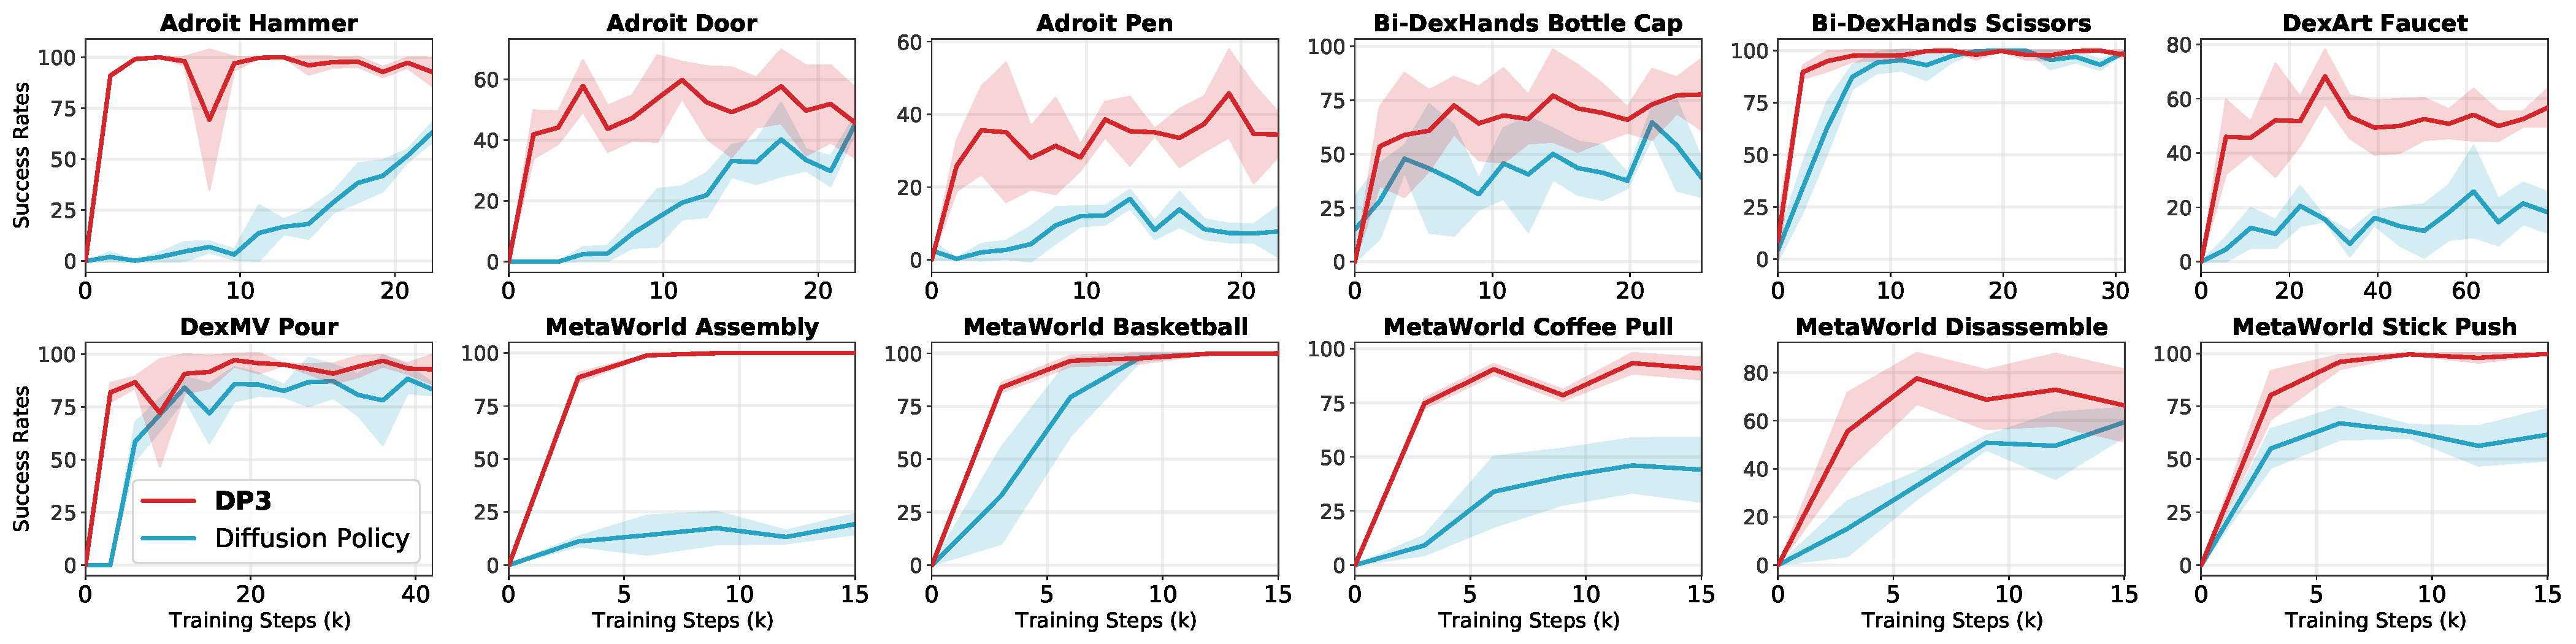
\includegraphics[width=0.96\textwidth]{figures/learning_efficiency_multi.pdf}
    \vspace{-0.1in}
    \caption{\textbf{Learning efficiency.} We sample 12 simulation tasks and show the learning curves of \ours and Diffusion Policy. \ours demonstrates a rapid convergence towards high accuracy. In contrast, Diffusion Policy exhibits a slower learning progress and achieves notably lower convergence in most tasks.}
    \label{fig:learning efficiency}
    \vspace{-0.15in}
\end{figure*}
\begin{figure*}[t]
    \centering
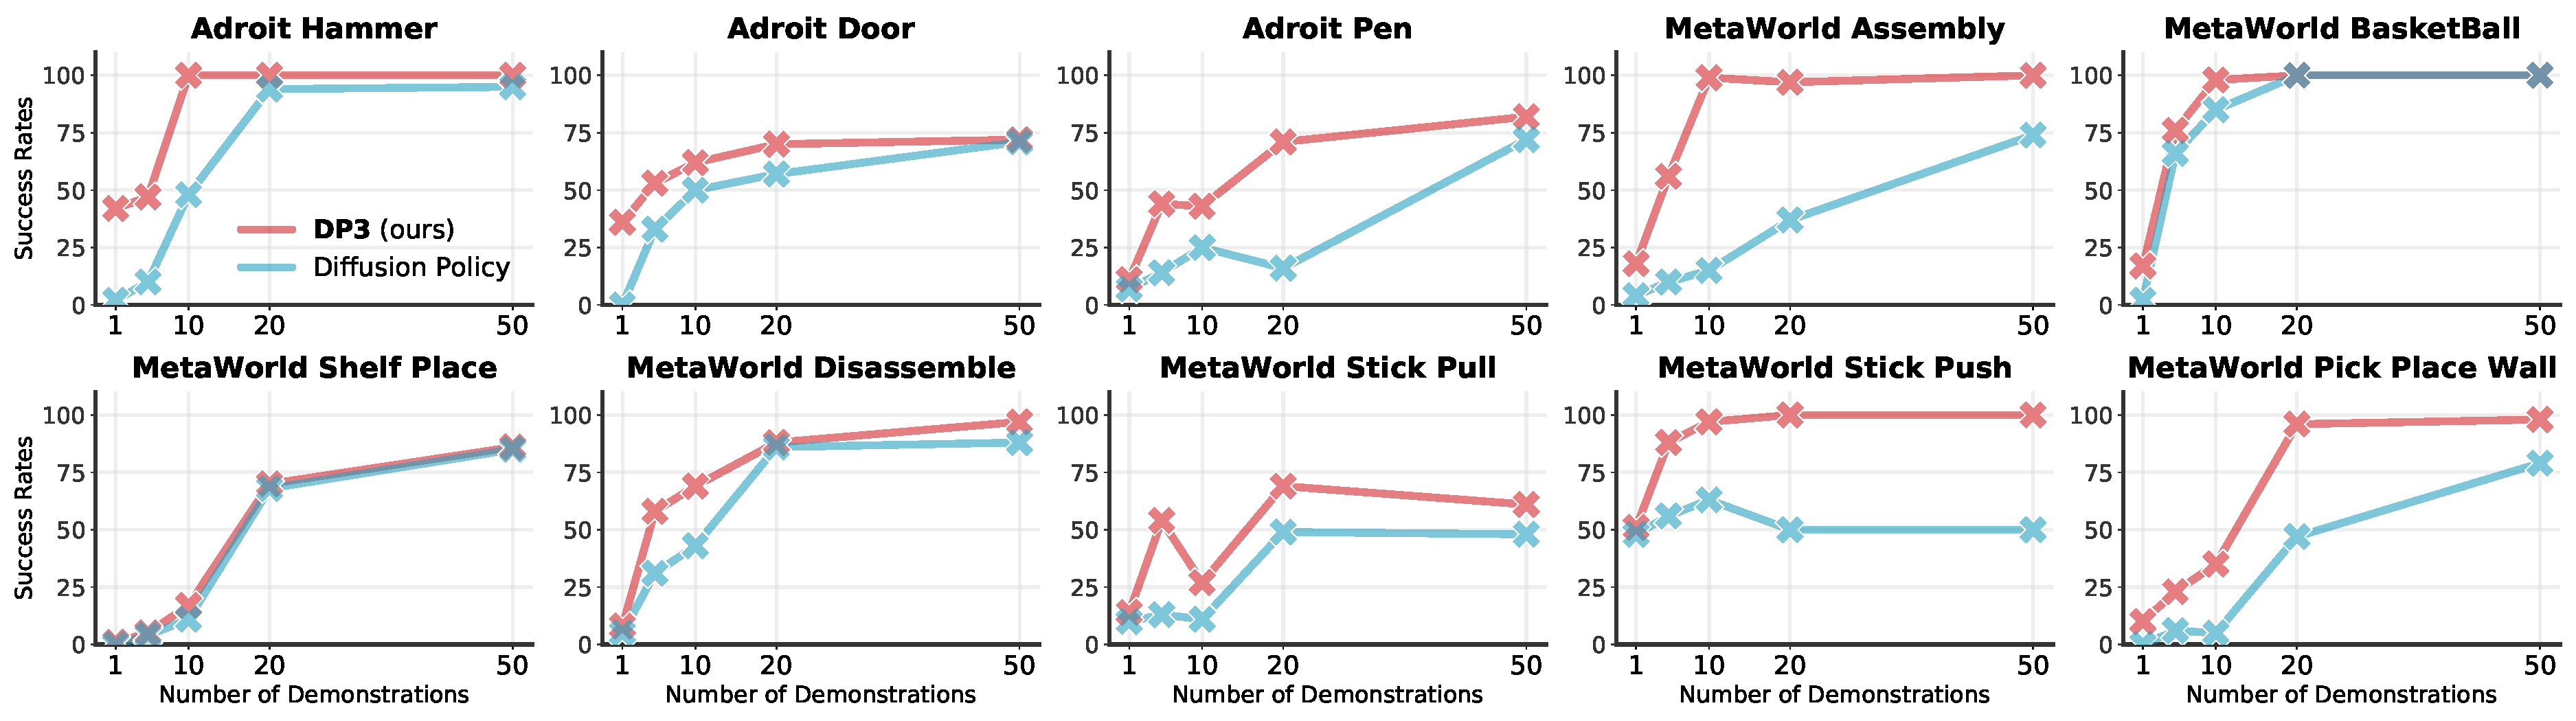
\includegraphics[width=0.96\textwidth]{figures/demo_scaling_multi.pdf}
\vspace{-0.1in}
    \caption{\textbf{Efficient scaling with demonstrations.} We sample 10 simulation tasks and train \ours and Diffusion Policy with an increasing number of demonstrations. \revise{
    \ours addresses all these tasks well and generally improves the accuracy with more demonstrations. Diffusion Policy also scales well on some tasks while still falling short of accuracy.}}
    \label{fig:demo scaling}
    \vspace{-0.25in}
\end{figure*}

\subsection{Efficiency and Effectiveness}
\ours shows surprising efficiency across diverse tasks, mainly reflected in the following three perspectives: 
\begin{enumerate}
    \item \textbf{High accuracy.} Summarized results are in Figure~\ref{fig:teaser}(a) and results for each domain are in Table~\ref{table:simulation simplified}. 
    We observe that DP3 achieves a success rate exceeding 90\% in nearly 30 tasks, whereas Diffusion Policy does in fewer than 15 tasks. Additionally, DP3 did not record any task with a success rate below 10\%, in contrast to Diffusion Policy, which had more than 10 tasks below 10\%. Note that most of the tasks are only trained with \textbf{10} demonstrations.
    \item \textbf{Learning efficiency.}
    While we train all the algorithms for 3000 epochs to guarantee convergence, we observe that \ours typically reaches convergence within approximately 500 epochs across all tasks, as illustrated in Figure~\ref{fig:learning efficiency}. In contrast, Diffusion Policy tends to converge at a much slower pace or converge into sub-optimal results.
    \item \textbf{Efficient scaling with demonstrations.} As shown in Figure~\ref{fig:demo scaling}, we find that in Adroit tasks, both \ours and Diffusion Policy perform reasonably while \ours achieves a comparable accuracy with fewer demonstrations. \revise{For some MetaWorld tasks above the \textit{easy} level such as Assembly and Disassemble, DP3 could achieve higher accuracy when demonstrations are sufficient.} This underscores that the 3D modality is not just beneficial but essential for certain manipulation tasks.
    % As shown in Figure~\ref{fig:demo scaling}, we find that in Adroit tasks, both \ours and Diffusion Policy perform reasonably while \ours achieves a comparable accuracy with fewer demonstrations. For MetaWorld tasks above the \textit{easy} level, Diffusion Policy fails to learn even with an increased number of demonstrations, lagging significantly behind \ours. This underscores that the 3D modality is not just beneficial but essential for certain manipulation tasks.
    \item \textbf{Competitive inference speed.} As depicted in Figure~\ref{fig:teaser}, \ours achieves an inference speed marginally surpassing Diffusion Policy. Contrary to the prevailing assumption that 3D-based policies are slower~\citep{shridhar2023peract,ze2023gnfactor,xian2023chaineddiffuser}, \ours manages to achieve efficient inference speeds, primarily attributed to the utilization of sparse point clouds and compact 3D representations.
\end{enumerate}








\subsection{Ablations}
We select 6 tasks to conduct more ablation studies: Hammer (\textbf{H}), Door (\textbf{D}), Pen (\textbf{P}) from Adroit and \revise{Assembly (\textbf{A}), Disassemble (\textbf{DA}),  Stick-Push (\textbf{SP})} from MetaWorld. These tasks include both high-dimensional and low-dimensional control tasks, and each task only uses 10 demonstrations. We use the abbreviations of these tasks in the tables for simplicity.
 



% \textbf{Number of points.} Shown in Table~\ref{table: number of points}.
% \begin{table}[htbp]
\centering
\caption{\textbf{Number of points for \ours.} }
\label{table: number of points}
\resizebox{0.49\textwidth}{!}{%
\begin{tabular}{l|cccccc|ccc}
\toprule

% & \multicolumn{3}{c}{\textbf{Adroit}} & \multicolumn{3}{c}{\textbf{MetaWorld}} \\
 % Algorithm & Hammer & Door  & Pen & Assembly & Basketball & Shelf Place & \textbf{Average} \\

  \# Points & H & D  & P & A & B & S & \textbf{Average} \\

\midrule

\textbf{512} & \dd{100}{0} &  \dd{62}{4} &  \dd{43}{6}  & \dd{49}{5} & \dd{91}{7} & \dd{34}{3}  \\
1024 & \dd{100}{0} &  \dd{59}{6} &  \dd{50}{4}  & \dd{}{} & \dd{}{}  & \dd{}{}   \\
2048 & \dd{100}{0} &  \dd{62}{5} &  \dd{49}{4}  & \dd{}{} & \dd{}{}  & \dd{}{}   \\


\bottomrule
\end{tabular}}
\end{table}






\textbf{Choice of 3D representations.} 
In \ours, we deliberately select point clouds to represent the 3D scene. To compare different choices of 3D representations,  we implement other 3D representations, including RGB-D, depth, and voxel. \revise{We also compare with oracle states, which include object states, target goals, and robot velocity besides robot poses.} The RGB-D and depth images are processed using the same image encoder as Diffusion Policy, while voxel representations employ the VoxelCNN, as implemented in \citep{chen2023visual_dex}. As demonstrated in Table~\ref{table: different 3D form}, these alternative 3D representations fall short of \ours. 
\revise{We note that RGB-D and depth images are close and not comparable to point clouds, indicating that the proper usage of depth information is essential. Additionally, we observe that point clouds and oracle states are very competitive, showing that point clouds might help learn an optimal policy from demonstrations.}





\begin{table}[htbp]
\centering
% \vspace{-0.1in}
\caption{\textbf{Ablation on 3D representations.} We replace the visual observation and the corresponding encoder in \ours to evaluate different 3D representations.}
\vspace{-0.05in}
\label{table: different 3D form}
\resizebox{0.49\textwidth}{!}{%
\begin{tabular}{l|cccccc|ccc}
\toprule


  Repr. & H & D  & P & A & DA & SP & \textbf{Average} \\

\midrule
\revise{Oracle State} & \dd{99}{2} & \dd{61}{2} & \ddbf{44}{3} & \dd{94}{1} & \ddbf{72}{7} & \dd{91}{8} & $76.8$ \\

\textbf{Point cloud} & \ddbf{100}{0} & \ddbf{62}{4} & \dd{43}{6} & \ddbf{99}{1} & \dd{69}{4} & \ddbf{97}{4} & \ccbf{78.3} \\


Image & \dd{48}{17} & \dd{50}{5} & \dd{25}{4} & \dd{15}{1} & \dd{43}{7} & \dd{63}{3} & $40.7$ \\

Depth & \dd{39}{15} & \dd{49}{1} & \dd{12}{3} & \dd{15}{4}  & \dd{15}{2} & \dd{62}{3} & $32.0$ \\



RGB-D & \dd{57}{14} & \dd{47}{5} & \dd{14}{2} & \dd{15}{3} & \dd{14}{1} & \dd{61}{3} & $34.7$\\

Voxel & \dd{54}{5} & \dd{33}{3} & \dd{18}{2} & \dd{10}{2} & \dd{17}{1} & \dd{62}{6} & $32.3$\\

\bottomrule
\end{tabular}}
\vspace{-0.1in}
\end{table}




\textbf{Choice of point cloud encoders.} We compare DP3 Encoder with other widely used point encoders, including PointNet~\citep{qi2017pointnet},  PointNet++~\citep{qi2017pointnet++}, PointNeXt~\citep{qian2022pointnext}, and Point Transformer~\citep{zhao2021point_transformer}. We also include the pre-trained models of PointNet++ and PointNeXt. Surprisingly, we find that none of these complex models and the pre-trained ones are competitive to DP3 Encoder, as shown in Table~\ref{table: different 3D encoder}.

% Though pre-trained encoders have been successful in 2D domains~\citep{yuan2022pieg}, it is not as useful for 3D domains.\ze{TBD: write this paragraph with more exps}

\begin{table}[htbp]
\centering
% \vspace{-0.1in}
\caption{\textbf{Ablation on point cloud encoders.} We replace DP3 Encoder with other widely used encoders, including PointNet~\citep{qi2017pointnet}, PointNet++~\citep{qi2017pointnet++}, PointNeXt~\citep{qian2022pointnext}, and Point Transformer~\citep{zhao2021point_transformer}. We also include the pre-trained encoders.}
\label{table: different 3D encoder}
\vspace{-0.05in}
\resizebox{0.49\textwidth}{!}{%
\begin{tabular}{l|cccccc|ccc}
\toprule



  Encoders & H & D  & P & A & DA & SP & \textbf{Average} \\


\midrule


\textbf{DP3 Encoder} & \ddbf{100}{0} & \ddbf{62}{4} & \ddbf{43}{6} & \ddbf{99}{1} & \ddbf{69}{4} & \ddbf{97}{4} & \ccbf{78.3} \\


PointNet & \dd{46}{8} & \dd{34}{8} & \dd{14}{4} & \dd{0}{0}& \dd{0}{0}& \dd{0}{0} &  $15.7$\\

PointNet++ & \dd{0}{0} & \dd{0}{0} & \dd{13}{3} & \dd{0}{0} & \dd{0}{0}& \dd{0}{0} & $2.2$ \\

PointNeXt & \dd{0}{0} & \dd{0}{0} & \dd{14}{3} & \dd{0}{0} & \dd{0}{0}& \dd{0}{0}  & $2.3$\\

Point Transformer & \dd{0}{0} & \dd{0}{0} & \dd{6}{5}& \dd{0}{0}& \dd{0}{0}& \dd{0}{0} & $1.0$ \\

PointNet++ (pre-trained) & \dd{5}{9} & \dd{19}{12} & \dd{17}{6}  & \dd{0}{0} & \dd{0}{0} & \dd{0}{0} & $6.8$ \\

PointNeXt (pre-trained) & \dd{0}{0} & \dd{36}{13} & \dd{17}{6} & \dd{0}{0} &\dd{0}{0}  &\dd{0}{0} & $8.8$\\

\bottomrule
\end{tabular}}
\vspace{-0.1in}
\end{table}



\textbf{Gradually modifying a PointNet.} To elucidate the performance disparity between DP3 Encoder and a commonly used point cloud encoder, \textit{e.g.}, PointNet, we gradually modify a PointNet to make it aligned with a DP3 Encoder. Through extensive experiments shown in Table~\ref{table: modify PointNet}, we identify that the T-Net and BatchNorm layers in PointNet are primary inhibitors to its efficiency.  By omitting these two elements, PointNet attains an average success rate of $72.3$, competitive to $78.3$ achieved by our DP3 Encoder.One plausible explanation for the T-Net is that our control tasks use the fixed camera and  do not require feature transformations from the T-Net. \revise{Further replacing high-dimensional features with a lower-dimensional one would not hurt the performance much ($72.5\rightarrow 72.3$) but increase the speed.} We would explore the reason for the failures of other encoders in the future.
\begin{table}[htbp]
\centering
% \vspace{-0.2in}
\caption{\textbf{Gradually modifying a PointNet to a DP3-style encoder.} Conv: use convolutional layers or linear layers. w/ T-Net: with or without T-Net. w/ BN: with or without BacthNorm layers. 1024 Dim: set feature dimensions before the projection layer to be 1024 or 256. Average success rates for 6 ablation tasks are reported.}
\label{table: modify PointNet}
\vspace{-0.05in}

% \resizebox{0.49\textwidth}{!}{%
% \begin{tabular}{l|cccccc|ccc}
% \toprule



%   Encoders & H & D  & P & A & DA & SP & \textbf{Average} \\


% \midrule



% PointNet & \dd{46}{8} & \dd{34}{8} & \dd{14}{4} & \dd{0}{0} & \dd{0}{0} & \dd{0}{0} & \\

% ~Linear & \dd{45}{6}& \dd{37}{5}& \dd{12}{2} & \dd{0}{0} & \dd{0}{0} & \dd{0}{0} & $15.7$\\

% ~Linear + D256 & \dd{47}{2} & \dd{45}{4}& \dd{16}{5}& \dd{0}{0} & \dd{0}{0} & \dd{1}{2} & $18.2$ \\

% ~w/o T & \dd{47}{3} & \dd{14}{6} & \dd{13}{2} & \dd{0}{0} & \dd{0}{0} & \dd{22}{21} & $16.0$ \\

% ~Linear + D256 + w/o BN & \dd{56}{4} & \dd{33}{3}& \dd{10}{3} & \dd{0}{0}& \dd{0}{0}& \dd{62}{9} & $26.8$\\

% ~Linear + w/o T & \dd{47}{8} & \dd{19}{6} & \dd{15}{4} & \dd{0}{0} & \dd{0}{0} & \dd{23}{20} & $26.0$ \\

% ~w/o T + Linear + D256 & \dd{49}{3} & \dd{16}{3} & \dd{14}{12} & \dd{0}{0}& \dd{0}{0}& \dd{0}{0}& $19.8$\\

% ~w/o BN + w/o T & \dd{100}{0} & \dd{50}{2} & \dd{44}{2} &  \dd{96}{3} & \dd{53}{10} & \dd{92}{2} & $72.5$ \\

% ~Linear + w/o BN + w/o T & \dd{100}{0}& \dd{50}{6}& \dd{43}{6}& \dd{97}{3}  & \dd{58}{13} & \dd{92}{2} & $73.3$ \\

% ~{Linear + D256 + w/o BN + w/o T} & \dd{100}{0}& \dd{56}{3}& \dd{41}{1}& \dd{95}{0} & \dd{50}{3} &\dd{92}{2} & $72.3$  \\

% \textbf{DP3 Encoder} & \dd{100}{0} & \dd{62}{4} & \dd{43}{6} & \\


% \bottomrule
% \end{tabular}}


\resizebox{0.48\textwidth}{!}{%
\begin{tabular}{c|cccc|ccccc}
\toprule



  Encoders & Conv& w/ T-Net & w/ BN & 1024 Dim& \textbf{Average} \\
  \midrule
PointNet & \textcolor{ggreen}{\Checkmark} & \textcolor{ggreen}{\Checkmark} & \textcolor{ggreen}{\Checkmark} & \textcolor{ggreen}{\Checkmark} & $15.7$ \\

 & \textcolor{gred}{\XSolidBrush} & \textcolor{ggreen}{\Checkmark} & \textcolor{ggreen}{\Checkmark} & \textcolor{ggreen}{\Checkmark} & $15.7$ \\

 & \textcolor{ggreen}{\Checkmark} & \textcolor{gred}{\XSolidBrush} & \textcolor{ggreen}{\Checkmark} & \textcolor{ggreen}{\Checkmark} &  $16.0$\\


  & \textcolor{gred}{\XSolidBrush} & \textcolor{gred}{\XSolidBrush}  & \textcolor{ggreen}{\Checkmark} & \textcolor{ggreen}{\Checkmark} & $26.0$ \\


     


& \textcolor{gred}{\XSolidBrush} & \textcolor{ggreen}{\Checkmark} & \textcolor{ggreen}{\Checkmark} & \textcolor{gred}{\XSolidBrush} & $18.2$\\

  Turnaroud! & \textcolor{ggreen}{\Checkmark}  & \textcolor{gred}{\XSolidBrush} & 
    \textcolor{gred}{\XSolidBrush} &\textcolor{ggreen}{\Checkmark} &  $\mathbf{72.5}$ \\



  & \textcolor{gred}{\XSolidBrush} & \textcolor{gred}{\XSolidBrush}  & \textcolor{ggreen}{\Checkmark} & \textcolor{gred}{\XSolidBrush} & $19.8$\\


& \textcolor{gred}{\XSolidBrush} & \textcolor{ggreen}{\Checkmark} & \textcolor{gred}{\XSolidBrush} & \textcolor{gred}{\XSolidBrush} & $26.8$\\





    
    & \textcolor{gred}{\XSolidBrush} & \textcolor{gred}{\XSolidBrush}  & \textcolor{gred}{\XSolidBrush} & \textcolor{gred}{\XSolidBrush} & $\mathbf{72.3}$\\


\bottomrule
\end{tabular}}
\vspace{-0.1in}
\end{table}








\textbf{Design choices in \ours.} Besides the 3D representations, the effectiveness of \ours is contributed by several small design choices, as shown in Table~\ref{table: ablation component}. (a) Cropping point clouds helps largely improve accuracy; (b) Incorporating LayerNorm layers could help stabilize training across different tasks~\citep{hansen2023tdmpc2,ba2016layer_norm}; (c) Sample prediction in the noise sampler brings faster convergence, also shown in Figure~\ref{fig:learning curve sample and epsilon}; (d) The projection head in DP3 Encoder accelerates the inference by projecting features to the lower dimension, without hurting accuracy; (e) Removing color channels ensures robust appearance generalization; (f) In low-dimensional control tasks, DPM-solver++~\citep{lu2022dpm_solver} as the noise sampler is competitive to DDIM, while DPM-solver++ could not handle high-dimensional control tasks well.


\begin{table}[htbp]
\centering
% \vspace{-0.05in}
\caption{\textbf{Ablation on design choices in \ours.} Most of the design choices would not affect the accuracy but bring other benefits such as appearance generalization by removing color.}
\label{table: ablation component}
\vspace{-0.05in}
\resizebox{0.49\textwidth}{!}{%
\begin{tabular}{l|cccccc|ccc}
\toprule

% & \multicolumn{3}{c}{\textbf{Adroit}} & \multicolumn{3}{c}{\textbf{MetaWorld}} \\
% Algorithm & Hammer & Door  & Pen & Assembly & Basketball & ShelfPlace & \textbf{Average} \\

 Designs & H & D  & P & A & DA & SP & \textbf{Average} \\

\midrule



\textbf{DP3}& \ddbf{100}{0} & \dd{62}{4} & \dd{43}{6} & \ddbf{99}{1} & \dd{69}{4} & \dd{97}{4} & \ccbf{78.3}  \\



w/o cropping & \dd{98}{1} & \ddbf{69}{3} & \dd{14}{1} & \dd{19}{9} & \dd{32}{6} & \dd{40}{2} &  $45.3$ \\


w/o LayerNorm & \ddbf{100}{0} & \dd{56}{4} & \dd{44}{3} & \dd{96}{2} & \dd{51}{3} & \dd{91}{5} &  $73.0$ \\

w/o sample pred &  \dd{68}{3} & 	\dd{67}{8} &	\dd{37}{12} & \dd{96}{2} & \dd{58}{9} & \dd{76}{9} & $67.0$ \\

w/o projection & \ddbf{100}{0} & \dd{61}{2} & \ddbf{47}{3} & \ddbf{99}{1} & \dd{60}{8} & \ddbf{99}{2} & $77.7$\\

w/ color & \ddbf{100}{1}	& \dd{67}{3}	& \dd{46}{4} & \dd{76}{8} & \ddbf{75}{5} & \dd{68}{3} & $72.0$ \\

DDIM$\rightarrow$DPM-solver++ & \dd{12}{4} & \dd{9}{5} & \dd{26}{5} & \dd{93}{3} & \dd{58}{6} & \dd{92}{14} & $48.3$  \\

\bottomrule
\end{tabular}}
\vspace{-0.05in}
\end{table}


\begin{figure}[htbp]
    \centering
    \vspace{-0.1in}
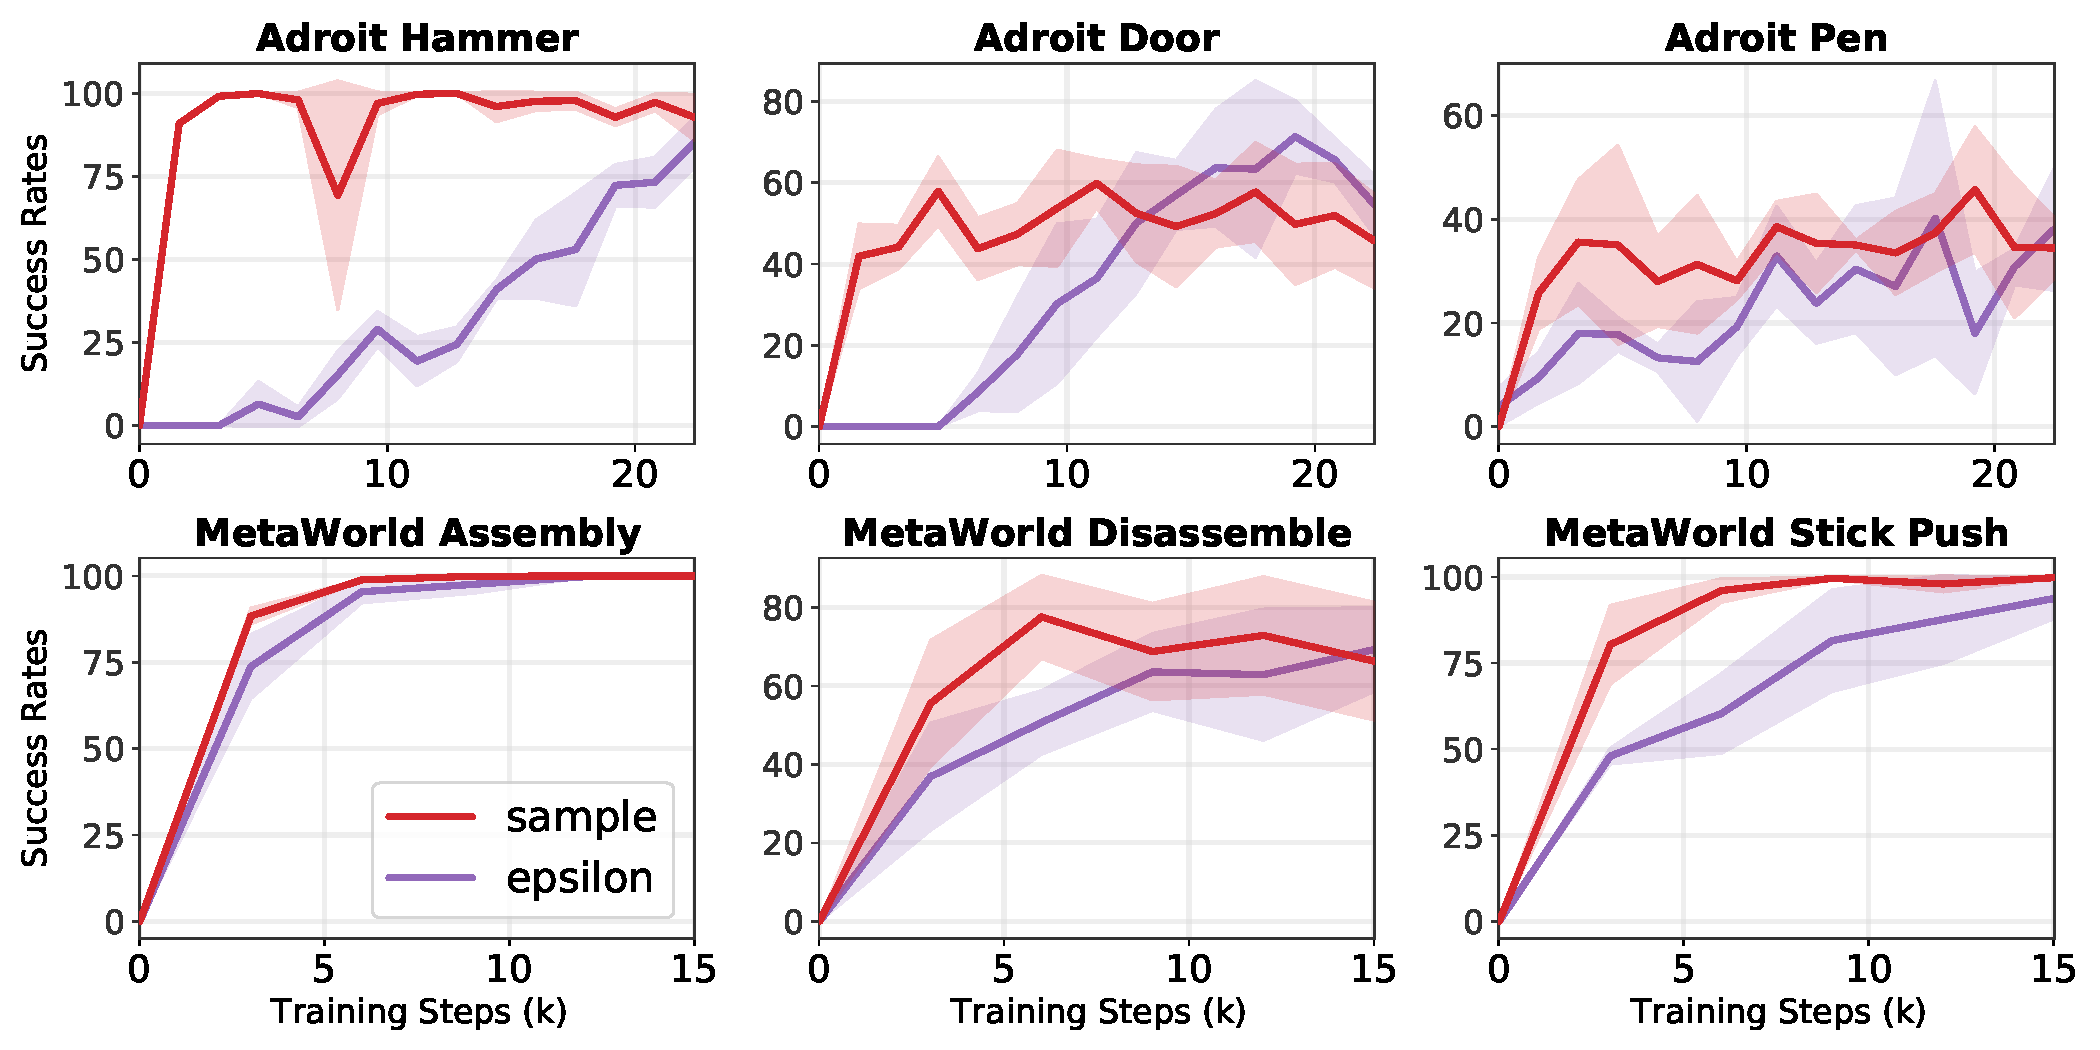
\includegraphics[width=0.48\textwidth]{figures/learning_curves_noise_pred.pdf}\vspace{-0.1in}
    \caption{\textbf{Learning curves of \ours with sample prediction and epsilon prediction.} With sample prediction, \ours generally converges faster, while epsilon prediction is also competitive.}
    \label{fig:learning curve sample and epsilon}
    \vspace{-0.1in}
\end{figure}








